After both processes our star's material is rich in neutrons, which are fermions, and therefore Pauli's exclusion principle applies to them too. Everything is the same as for electrons, the only difference being that they have a different \(\lambda_{DB}\). A similar analysis to electrons can be done with two differences: using the neutron mass instead of the electron's, and setting \(Z/A=1\). This results in
\begin{align}
    R_{ns} = \qty{2.3e9}{}\frac{m_e}{m_n}\ins{\frac{M}{M_\mathSun}}^{-1/3} = \qty{11}{\kilo\meter}\ins{\frac{M}{M_\mathSun}}^{-1/3}
\end{align}
which is about 500 times smaller than a white dwarf. The density in comparison to a white dwarf will be
\begin{equation}
    \frac{\rho_{ns}}{\rho_{wd}} \sim 500^3 \sim \qty{e8}{} \implies \rho_{ns} \sim \qty{e14}{\gram\per\centi\meter^3}
\end{equation}
If we look at the density of material in the nucleon of an atom it is
\begin{equation}
    \rho_{nuc} = \frac{m_p}{\frac{4\pi}{3}\ins{\qty{1}{\femto\meter}}^3}\sim \qty{4e14}{\gram\per\centi\meter^3}
\end{equation}
So the density of a neutron star is in comparable to that of the nucleus of an atom. You could think of the entire thing as a single atom nucleus with atomic number \(\qty{e57}{}\). Recalling the expression for \(M_{ch}\):
\begin{equation}
    M_{ch} = 0.21 \ins{\frac{Z}{A}}^2\alpha_G^{-3/2}m_p
\end{equation}
setting the relation we had for neutron stars
\begin{equation}
    M_{ns}=0.21\alpha_G^{-3/2}m_p = 5.6M_\mathSun
\end{equation}
which is the upper limit for the mass of a neutron star. A neutron star more massive than that won't hold itself together and collapse further. Observations indeed haven't found any neutron stars heavier than (or even close to) that mass. More accurate calculations give a result significantly lower. The reason for this is that general relativistic effects become important at this scale. Relativistic effects become relevant when
\begin{equation}
    \frac{E_{Gr}}{mc^2}\sim\frac{\frac{GM_{ns}m}{R_{ns}}}{mc^2}=\frac{GM_{ns}}{R_{ns}c^2}\sim 0.2
\end{equation}
Another important effect we haven't mentioned yet is the strong nuclear force. Since the neutron star effectively behaves like a giant nucleus, the strong force will start to have an effect. We don't quite understand what its effect is though. If we want to look at how much energy is expected to be released in the collapse of a core into a neutron star
\begin{equation}
    \Delta E_{gr} = \left\lvert\frac{\frac{3}{5}GM^2}{R_0}-\frac{\frac{3}{5}GM^2}{R_{ns}}\right\rvert \approx \frac{\frac{3}{5}GM^2}{R_{ns}}
\end{equation}
and if we insert typical quantities for neutron stars
\begin{align}
    M=1.3M_\mathSun && R_{ns} = \qty{11}{\kilo\meter}
\end{align}
we find
\begin{equation}
    \Delta E_{gr} \sim \qty{3e53}{\erg}
\end{equation}
This energy has to go somewhere and this causes a supernova. This is the leading process which causes supernovas. This kind of supernova is called a core-collapse supernova. The luminosity we see from this process is

\begin{figure}[!htb]
    \centering
    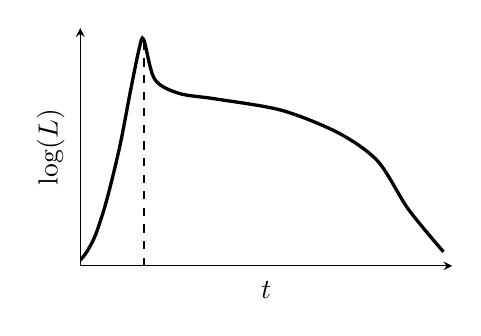
\begin{tikzpicture}
        \begin{axis}[
            width=0.52\linewidth,
            height=4.6cm,
            axis lines=left,
            xmin=0, xmax=8.5,
            ymin=0, ymax=4.2,
            xtick=\empty,
            ytick=\empty,
            xlabel={$t$},
            ylabel={$\log(L)$},
        ]
            % Schematic light-curve shape (immediate rise, sharp peak, long tail)
            \addplot[very thick, smooth] coordinates {
                (0.0,0.10)
                (0.15,0.25)
                (0.35,0.55)
                (0.60,1.15)
                (0.90,2.10)
                (1.15,3.10)
                (1.35,3.85)
                (1.45,4.00)
                (1.70,3.30)
                (2.25,3.05)
                (3.10,2.95)
                (4.60,2.75)
                (5.90,2.35)
                (6.80,1.85)
                (7.50,1.00)
                (8.30,0.25)
            };

            % Peak marker
            \addplot[thick, dashed] coordinates {(1.45,0) (1.45,4.05)};
            \node[below] at (axis cs:1.45,0) {$t_{\mathrm{peak}}$};
        \end{axis}
    \end{tikzpicture}
    \caption{Schematic supernova light curve (log-luminosity vs. time) with a peak time $t_{\mathrm{peak}}$. (Converted from a whiteboard drawing using OpenAI Prism)}
\end{figure}

and the total energy we observe is
\begin{equation}
    E_\gamma = \int \dd t L = \qty{3e49}{\erg}
\end{equation}
which is only \( 0.01\% \) of the available energy. Where does the rest of the energy go? Maybe it is ejected from the supernova. The ejected mass is about \(\ins{1-10}M_\mathSun \) and observations show that its velocity is \(v\sim\qty{e4}{\kilo\meter\per\second}\). This gives us an energy of
\begin{equation}
    E_{k} \sim \frac{1}{2}M_{ej}v^2 = \qty{3e51}{\erg}
\end{equation}
which is \(1\% \) of the total energy, so there must be another explanation. Approximately \(99\% \) is ejected as neutrinos. The density in the center of the supernova is extremely high and the temperature is very high, which means there are very many photons whizzing around close to each other, and some of them collide with each other which results in
\begin{equation}
    \gamma + \gamma \rightarrow e + e^+ \rightarrow \begin{cases}
        \nu_e + \overline{\nu}_e \\
        \nu_\mu + \overline{\nu}_\mu \\
        \nu_\tau + \overline{\nu}_\tau
    \end{cases}
\end{equation}
The conditions are so extreme that sometimes even the neutrinos go through collision processes. The reason this process doesn't happen in the sun is that there just isn't enough energy there. The rest energy of the electron is \(m_{e}c^2 = \qty{0.5}{\mega\electronvolt}\) which photon collisions can't reach in the sun. Other types of explosions: Type 1a supernovae. There's a white dwarf just chilling on its own but a red giant approaches it and the white dwarf starts accreting material from the red giant. It then eventually reaches \(M_{ch}\) and explodes. In regular stars there is a negative feedback loop where fusion causes temperature to increase, which increases the pressure, which increases the radius of the star, which lowers the temperature, which lower the rate of fusion. In contrast in a white dwarf fusion causes an increase in temperature which doesn't affect the pressure, so it increases the rate of fusion again, and so on. This is called a type 1a supernova. Another kind of explosion is a gamma ray burst. The energy released from GRBs is \(E\sim\qty{e51}{\erg}\) which is all released over about 0.1 seconds to a minute. GRBs are an active research area and it's theorized that there are several types.